\documentclass[border=4pt]{standalone}
\usepackage{tikz}
\usetikzlibrary{arrows.meta,positioning,shapes.geometric}
\begin{document}
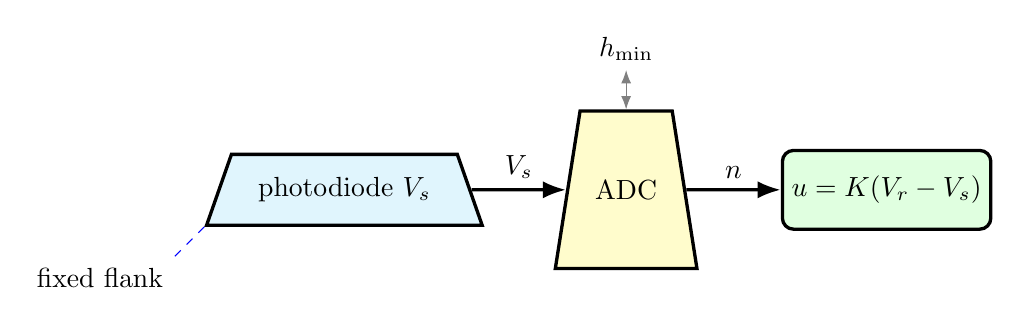
\begin{tikzpicture}[>=Latex,node distance=12mm]
  \node[
    trapezium,
    trapezium stretches body,
    trapezium angle=60,
    draw,
    very thick,
    fill=cyan!12,
    minimum width=35mm,
    minimum height=9mm
  ] (sensor) {photodiode $V_s$};

  \node[
    trapezium,
    trapezium stretches,
    trapezium angle=60,
    draw,
    very thick,
    fill=yellow!20,
    minimum width=18mm,
    minimum height=20mm,
    right=of sensor
  ] (adc) {ADC};

  \node[draw,very thick,rounded corners,fill=green!12,right=of adc,
    minimum width=25mm,minimum height=10mm] (controller) {$u=K(V_r-V_s)$};

  \draw[-Latex,very thick] (sensor.right side) -- node[above] {$V_s$} (adc.left side);
  \draw[-Latex,very thick] (adc.right side) -- node[above] {$n$} (controller.west);
  \draw[<->,gray] (adc.top side) -- ++(0,5mm) node[above,black] {$h_{\min}$};
  \draw[dashed,blue] (sensor.bottom left corner) -- ++(-4mm,-4mm)
    node[below left,black] {fixed flank};
\end{tikzpicture}
\end{document}
